
\chapter{DISCUSSÃO DE RESULTADOS} 

	\par O sistema operacional \textit{Android} mostrou o porquê de ser tão
utilizado nos dias atuais. Com uma gama enorme de recursos totalmente gratuitos
e com a documentação excelente torna-se claro o que cada função realiza, com
decorrer do desenvolvimento do aplicativo.

	\par Como se constatou que os discentes, na maioria das vezes, acessam o portal
do aluno para consultar notas, faltas e provas agendadas, o aplicativo tem como
importância facilitar para que os graduandos tenham suas informações de maneira
simples e rápida. É notório que há mais facilidade em acessar esses dados pelos
\textit{smartphones} do que em \textit{desktops}, pois, quando um professor
lançar uma determinada nota, o aluno será notificado de que alguma informação
nova está no portal, evitando que o usuário fique entrando no portal várias
vezes ao dia ansioso em saber sua média final.
	
	\par O aplicativo é de fácil utilização, pois tem como tela principal, uma
\textit{activity} do tipo \textit{Navigation Drawer Layout}, que de acordo com
o \citeonline{android2015}, a \textit{activity} fica escondida e aparece somente quando
chamada pelo usuário exibindo do lado esquerdo do dispositivo todas as opções
de navegação do \textit{software}, facilitando para o aluno se localizar, além
de ficar com uma aparência mais agradável. A seguir pode-se ver na Figura
\ref{fig:dr1} o layout de menus que aparecerá quando clicado na opção
selecionada.
 

\begin{figure}[h!]
	\centerline{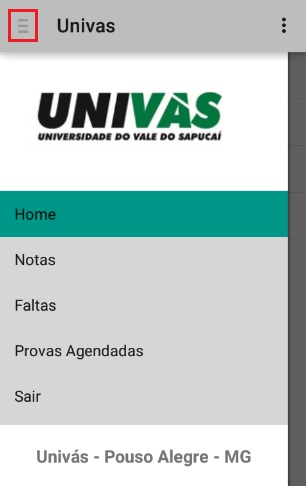
\includegraphics[scale=0.5]{./imagens/3_discussao_resultados/dr1.png}}
	\caption[Menu do Aplicativo]{Menu do Aplicativo.
		\textbf{Fonte:}Elaborado pelos autores.}
	\label{fig:dr1}
\end{figure}
\pagebreak

	\par Na \textit{home} do aplicativo foi utilizado uma lista com \textit{links}
 de \textit{sites} uteis aos alunos, como é visível na Figura \ref{fig:dr2}.
 Anteriormente havia se pensado em abrir os sites através de uma
 \textit{intent} implícita que como ressalta \citeonline{monteiro2012} é criada
 para avisar o sistema operacional \textit{Android}, que é necessário abrir uma
 outra \textit{activity}, a qual seria responsável por executar uma determinada
 ação, no caso, abrir uma página \textit{web}. Porém, decidiu-se usar o
 \textit{widget webView} que ainda segundo \citeonline{monteiro2012} permitirá
 carregar o \textit{site} no próprio aplicativo. Portanto, ao clicar em alguma
 dessas opções será aberta a \textit{activity} que detalhará o item, evitando
 abrir o navegador nativo, conforme é mostrado na Figura \ref{fig:dr3}.

\begin{figure}[h!]
	\centerline{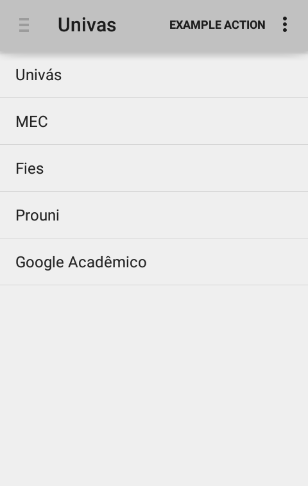
\includegraphics[scale=0.4]{./imagens/3_discussao_resultados/dr2.png}}
	\caption[\textit{Home} do Aplicativo]{\textit{Home} do Aplicativo.
		\textbf{Fonte:}Elaborado pelos autores.}
	\label{fig:dr2}
\end{figure}	

\begin{figure}[h!]
	\centerline{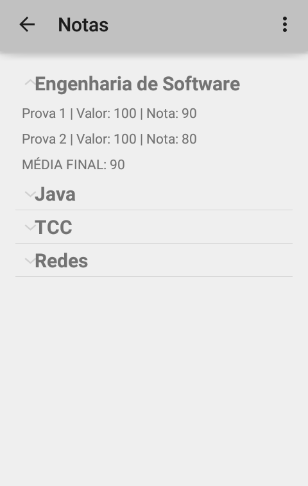
\includegraphics[scale=0.4]{./imagens/3_discussao_resultados/dr3.png}}
	\caption[\textit{Site} carregado no \texttt{webView}]{\textit{Site} carregado no \texttt{webView}.
		\textbf{Fonte:}Elaborado pelos autores.}
	\label{fig:dr3}
\end{figure}
\pagebreak	

	\par As informações dos alunos vem do \textit{web service} e são salvas no
banco de dados \textit{SQLite}, que conforme \citeonline{monteiro2012} é um
banco de dados que já vem na plataforma \textit{Android}, o qual não necessita
a instalação ou configuração de ferramentas externas. Logo após as notas, faltas
e provas agendadas são apresentadas aos usuários através de uma lista do tipo
\texttt{ExpadableListView}, este, segundo \citeonline{android3} traz a vantagem
que quando clicado em um de seus itens, é apresentado seus subitens na mesma
tela, evitando abrir uma nova \textit{activity} e com isso simplificando e
melhorando o desempenho do software. Abaixo, na Figura \ref{fig:dr4} é possível
ver a activity de notas, listando algumas informações com \textit{widget}
\texttt{ExpadableListView}.

\begin{figure}[h!]
	\centerline{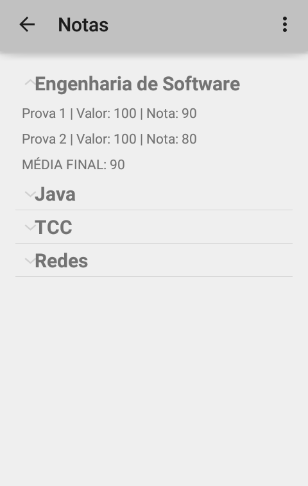
\includegraphics[scale=0.5]{./imagens/3_discussao_resultados/dr4.png}}
	\caption[Tela de Apresentação de notas, faltas e provas agendadas]{Tela de
	Apresentação de notas, faltas e provas agendadas.
		\textbf{Fonte:}Elaborado pelos autores.}
	\label{fig:dr4}
\end{figure}

%----------------------------------------------------------------------------------

	\par O aplicativo resultado desta pesquisa, tinha necessidade de consumir
dados para posteriormente apresentá-los ao usuário. Era necessário que, os
dados do sistema acadêmico da instituição de ensino que serviu como contexto
para esta pesquisa, fossem transmitidos de alguma forma ao aplicativo. Era
necessário também que os dados chegassem ao aplicativo respeitando as
particularidades de cada usuário, trazendo somente informações relevantes aos
mesmos. Com esse intuito de disponibilizar informações já citadas
anteriormente, a quem quer que fosse necessário, inclusive aos usuários do
aplicativo, foi criado um \textit{Web Service} REST. Este foi um dos resultados
alcançados através desta pesquisa.
	
	\par A construção do \textit{web service}, de ínicio, mostrava-se um tanto
quanto custosa, devido a restrições das tecnologias que foram escolhidas. Por se
tratar de uma simples \textit{web service} que seria disponibilizado para suplir
a demanda de dados do aplicativo, os primeiros serviços foram construídos e
disponibilizados fazendo uso de \textit{servlets} simples e conexão
JDBC\footnote{JDBC - \textit{Java Database Connectivity}}. Este modo como foi
pensado inicialmente, era simples de ser contruído e de uma
\textit{performance} aceitável. 

	\par Porém de acordo com o crescimento da demanda do serviço, tornou-se
inviável a contrução do mesmo com estas técnologias, devido a complexidade com
que era necessário contruir os serviços, haja vista que, com estas técnologias
era necessário que se fosse configurado praticamente tudo de forma manual
inclusive tratamento de erros da aplicação, respostas as requisições e tipos de
dados. Esta etapa teve, portanto, um resultado não muito amigável do ponto de
vista de sua construção. No entanto se for analizado do ponto de vista do
conhecimento adquirido, obteve-se um resulatdo satisfatório, pois, foi na
pesquisa e na busca melhores alternativas a estas técnologias, que se chegou ao
resultado final.

	\par O \textit{web service} foi desenvolvido com algumas técnolgias que
facilitaram a sua construção. Foi usado o \textit{framework Jersey} para prover
os serviços necessários. Este \textit{framework} usa \textit{servlets} para
disponibilizar os serviços, porém com a facilidade de já ter embutido em si o
tratamento para qualquer um dos tipos de midias que foram usadas na
implementação de um serviço REST, tanto para entrada ou saida de dados. Foi
ainda usado o \textit{framework} de pesistência de dados \textit{Hibernate}.
Este por sua vez desenpenhou papel notório, pois, ao mesmo tempo que facilitou
o desenvolvimento do \textit{web service} com relação ao foco nas regras de
negócio da aplicação e não tanto na implementação, pode-se dizer que se, por
algum motivo for necessário migrar de banco de dados este será um fator
facilitador. O resultado final foi extremamente satisfatório, pois era notório
que era facíl tanto contruir e disponibilizar um novo serviço, quanto consumir
o mesmo.
	
	\par Portanto, conclui-se que se for analizado estes resultados citados de
forma conjunta, pode-se dizer que o resultado geral foi satisfatório, pois, os
discentes puderam obter as informações de que mais fazem uso de forma prática e
rápida.


